%-------------------------------------------------%
\documentclass[12pt,oneside]{book}
%-------------------------------------------------%
\usepackage[spanish]{babel}
\usepackage[margin=1in]{geometry}
\usepackage{graphicx}
\usepackage{amssymb,amsmath,amsthm,amsfonts}
\usepackage{enumerate}
\usepackage{lipsum}
\usepackage{color}
\usepackage{float}
\usepackage{parskip}
\usepackage{titlesec}
\usepackage{apacite}
\usepackage{hyperref}
%-------------------------------------------------%
\titleformat{\chapter}{\normalfont\huge}{\thechapter.}{20pt}{\huge \bf}
\renewcommand{\qedsymbol}{\rule{0.7em}{0.7em}}
\providecommand{\abs}[1]{\lvert#1\rvert}
\graphicspath{ {Img/} }
\decimalpoint
%-------------------------------------------------%
\title{Tarea 1 - Optimización Lineal}
\author{}
\date{\today}
%-------------------------------------------------%
\begin{document}
\maketitle

\tableofcontents

\chapter{Teoría}

\section[Ejercicio]{}
{\large Defina brevemente qué 
es una función continúa 
y dé un ejemplo de una función que cumpla 
la definición y uno de una función que no la cumpla.}

\textit{Una función $f:A \rightarrow \mathbb{R}, \quad A \subseteq \mathbb{R}$ es continúa en $c$ si $\lim_{x \rightarrow c} f(x) = f(c)$, por lo que $f$ es continúa si cumple lo anterior $\forall c \in \mathbb{R}$.}

\textit{La función $f(x) = x^3-2x^2+5x-8$ es una función polinómica, la cual es continua en $\mathbb{R}$.}

\textit{La función $f(x) = \sqrt{1-x^2}$ no cumple la definición para valores distintos a $[-1,1]$.}

\section[Ejercicio]{}
{\large Defina brevemente qué es una función diferenciable y dé un ejemplo de una
función que cumpla la definición y uno de una función que no la cumpla.}

\textit{Una función $f:A \rightarrow \mathbb{R}, \quad A \subseteq \mathbb{R}$ es diferenciable en $c$ si es continua en $A$ y el limite}
\begin{equation*}
    \lim_{h \rightarrow 0} \frac{f(c+h)-f(c)}{h}
\end{equation*}
\textit{existe.}

\textit{La función $f(x) = 2x^4$  es diferenciable en $c = 3$}

\textit{La función $f(x) = \abs{x}$ no es diferenciable en $c = 0$}

\newpage

\section[Ejercicio]{}
{\large Defina brevemente qué es una función lineal y mencione el tipo de fenómenos que éstas modelan.}

\textit{La función lineal es un tipo de función polinómica de grado uno la cual comúnmente representamos como}
\begin{equation*}
    f(x)=mx+b
\end{equation*}
\textit{donde $m$ es la pendiente siendo $m \neq 0$ y $b$ la ordenada al origen.}

\textit{Estas funciones generalmente representan modelos de movimiento o fenómenos constantes, es decir que disminuyen o aumentan de manera constante y no variable, un ejemplo puede ser la velocidad de algún objeto en movimiento constante entre otros.}

\section[Ejercicio]{}
{\large Defina brevemente qué es una función no lineal y mencione el tipo de fenómenos que éstas modelan.}

\textit{Análogo al inciso anterior, una función no lineal son todas aquellas funciones tal que $f$ no es polinómica de primer grado}

\textit{Estas funciones modelan fenómenos más complejos, aquellos donde no representamos cambios constantes.}

\section[Ejercicio]{}
{\large  Dé tres ejemplos de funciones no lineales.}

\textit{Ejemplos de funciones no lineales:}

\begin{enumerate}
    \item $f(x) = \sin{x^2}$
    \item $g(x) = \sqrt{x^3+5}$
    \item $h(x) = \frac{1}{x}$
\end{enumerate}

\chapter{Programación}

\section[Ejercicio]{}
{\large Explique brevemente las diferencias, ventajas y desventajas entre un lenguaje de programación compilado y un lenguaje de programación interpretado.}

\subsection{Diferencias}
El lenguaje compilado requiere como paso adicional antes de ser ejecutado la compilación, que es en pocas palabras convertir el lenguaje usado a lenguaje maquina y después ejecutarlo, en cambio un lenguaje interpretado se convierte a lenguaje maquina conforme se va ejecutando.

\subsection{Lenguaje Compilado}
\subsubsection*{Ventajas}
\begin{enumerate}
    \item Se puede compilar una sola vez y ejecutarlo en cualquier momento
    \item Son más eficientes pero difíciles de depurar
\end{enumerate}
\subsubsection*{Desventajas}
\begin{enumerate}
    \item No se puede ejecutar hasta que el programa este libre de errores
    \item El programa ocupa más espacio porque todo el código reside en la memoria
\end{enumerate}

\subsection{Lenguaje Interpretado}
\subsubsection*{Ventajas}
\begin{enumerate}
    \item Es posible informar los errores en cuanto se encuentra el primero, facilita la observación de errores
    \item Puede ejecutarse por partes lo cual facilita su manejo y ejecución por partes
\end{enumerate}

\subsection*{Desventajas}
\begin{enumerate}
    \item Son menos eficientes, ocupan más tiempo en ejecutar
    \item Es más probable que el código se ejecute con nuevos errores cada vez que se quiera usar si no se verifica por completo
\end{enumerate}

\section[Ejercicio]{}
{\large Genere con Matlab dos matrices con entradas aleatorias entre cero y 100,
10x10, y súmelas ahí mismo muestre en su reporte tanto las matrices
generadas como la salida obtenida por el programa, con una captura de
pantalla}

\textit{Código}

\begin{figure}[H]
    \centering
    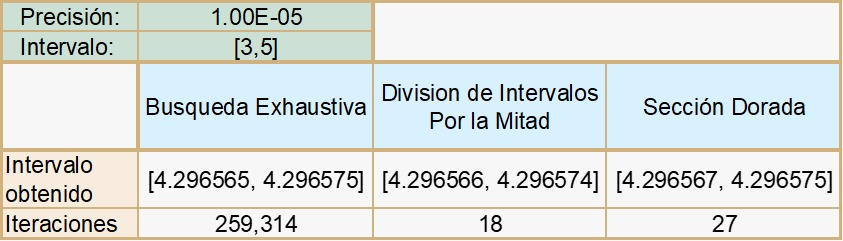
\includegraphics[width = 0.5\textwidth]{figura1}
\end{figure}

\newpage

\textit{Salida}

\begin{figure}[H]
    \centering
    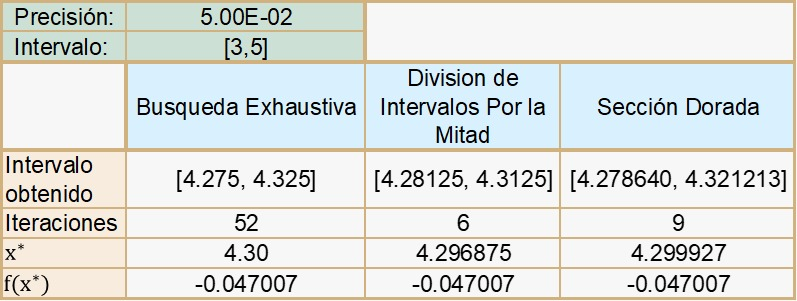
\includegraphics[width = 1\textwidth]{figura2}
\end{figure}

\section[Ejercicio]{}
{\large Escriba código en Matlab para aproximar numéricamente (mediante diferencias finitas) la derivada y la segunda derivada de la función}

\begin{equation*}
    f(x)=3^3+4x^2+2x, \quad \text{Evaluada en el punto} \quad x_0=7.
\end{equation*}

\textit{Código}

\begin{figure}[H]
    \centering
    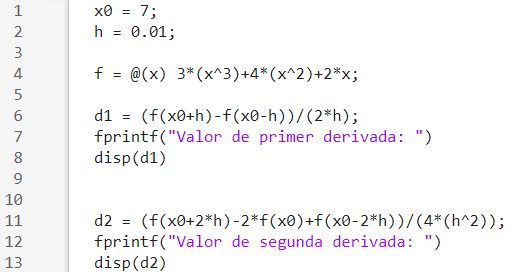
\includegraphics[width = 0.5\textwidth]{figura3}
\end{figure}

\textit{Salida}

\begin{figure}[H]
    \centering
    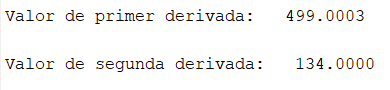
\includegraphics[width = 0.5\textwidth]{figura4}
\end{figure}



\chapter{Investigación}

\section[Ejercicio]{}

{\large Lea y Conteste detalladamente, y con sus propias palabras, a las siguientes
preguntas. Puede ayudarle leer el capítulo 1 de [Nocedal and Wright, 1999],
o la introducción de algún otro libro de Optimización.
}

\subsection{Describa de manera clara cuál es la importancia de la optimización
en ingeniería.}

Hacer y mejorar la eficiencia de los procesos necesarios así como minimizar los gastos y uso de material manteniendo el mismo resultado. 

\subsection{¿Qué elementos definen un problema de optimización?}

Aquellos aspectos que se quieran mejorar o usar de forma más eficiente como los recursos disponibles, los gastos, la mano de obra, etc. 

\subsection{¿Cómo se clasifica un problema de optimización?}

Este puede ser lineal o no lineal, puede contar o no con restricciones, ser continuo o discreto, y estar sujeto a un rango o ser global.

\newpage 

\section[Ejercicio]{}

{\large Describa brevemente dos aplicaciones de la vida real, donde se requiera
resolver un problema de optimización no lineal. Discuta la naturaleza no
lineal de estos problemas.}

\begin{itemize}
    \item Un ejemplo sería calcular el volumen máximo de un paquete de correo con base cuadrada y la anchura  mas la altura es fija. No es lineal ya que tendremos funciones de mayor grado gracias a que es volumen.
    \item Otro ejemplo es encontrar las dimensiones de un cartel que minimizan en el área del mismo para que cierto texto de área especifica con márgenes definidos entre como debería sin gastar más área de la necesaria.
\end{itemize}

\section[Ejercicio]{}

{\large Liste aquí las fuentes bibliográficas, al menos una, a la que tendrá acceso
durante el curso. Indicar si cuenta con el libro por préstamo de alguna
biblioteca, si lo tiene en formato electrónico, etc.}

\begin{itemize}
    \item Nocedal and Wright, 1999. Numerical optimization. Springer verlag. \textit{Libro en PDF}
    \item Hillier F. and Lieberman G. 1989. introducción  a la Investigación de operaciones. MacGraw-Hill. \textit{Libro en PDF}
\end{itemize}


\chapter{Referencias}

\begin{itemize}
    \item EcuRed. (n.d.). Funciones Continuas. EcuRed. Retrieved August 18, 2022, from \url{https://www.ecured.cu/Funciones_continuas}.
    \item Omniascience scholar. Catalog | OmniaScience Scholar. (n.d.). Retrieved August 19, 2022, from \url{https://www.omniascience.com/books/index.php/scholar/catalog/download/40/182/198-1?inline=1}
\end{itemize}

\end{document}